%!TEX program=luatex

\newpage
\pagenumbering{arabic}
\section{Introduction}
Avec la montée du Web 2.0, la production de contenu participatif et collaboratif a largement remplacé les méthodes traditionnelles de partage de l'information. Un vaste potentiel inexploité réside dans les quantités de données à la fois énormes et dynamiques disponibles sur les différentes plate-formes numériques qui ne peuvent être traités avec les méthodes de l'informatique classique.

\textcolor{red}{Les revues de presses, les blogs et les magazines représentent une partie considérable dans ce tsunami informationnel, et le choix des lectures quotidiennes devient de plus en plus difficile.}

Dans ce chapitre, nous allons discuter du Traitement Automatique du Langage Naturel (TALN), de sa puissance et son importance.\

En bref, l'objectif de cette partie est de décrire le but, les procédures et les applications pratiques du TALN d'une manière simple et claire. Nous examinerons la littérature la plus récente tout en décrivant les méthodes et les processus disponibles, nous analyserons certains des défis auxquels les chercheurs sont confrontés, et passerons brièvement en revue certaines des applications actuelles et futures de cette science.

\section{Définition}
Le Traitement automatique du langage naturel est l'un des principaux domaines de l'intelligence artificielle. Il permet de développer des systèmes qui peuvent \emph{analyser} et \emph{comprendre} le langage humain. En dehors des opérations courantes de traitement de texte qui considèrent les textes comme une simple séquence de symboles, l'utilisation des techniques de TALN permet d'organiser et de structurer des quantités énormes de connaissances pour développer des applications très avancées telles que la synthèse automatique, la reconnaissance d'entités, l'analyse des sentiments, la reconnaissance de la parole, etc.\\

Le TALN est considéré comme un problème difficile en informatique dû à l'imprécision du langage humain. Comprendre le langage humain, c'est comprendre non seulement les mots, mais aussi les concepts et comment ils sont liés pour créer du sens. Bien que la langue soit l'une des tâches les plus faciles à apprendre pour les humains, l'ambiguïté rend le traitement de cette dernière difficile à maîtriser pour les ordinateurs.

\section{Domaines d'application}
Le TALN est utilisé pour manipuler le langage humain, qu'il s'agisse d'extraire du sens ou de générer du texte dans le but d'accomplir des tâches telles que le résumé automatique d'un document, la traduction entre deux langages naturels ou la détection des spams.

On peut distinguer deux grands domaines où les techniques du TALN ont pu faire des avancés énormes: la \emph{recherche scientifique} et \emph{l'industrie informatique}.\\
%Recherche scientifique
Dans les laboratoires de recherche en intelligence artificielle, le TALN est considéré, souvent, comme l'une des branches les plus importantes et les plus productives.\\ 
De nombreuses activités cognitives qui se produisent dans l'esprit humain ont pu être simulées grâce à ses techniques.
On peut en citer quelques unes: 
\begin{itemize}
    \item \textbf{La traduction automatique:}
    la traduction automatique des textes est probablement l'un des domaines les plus connus de l'IA. Elle a fait l'objet de plusieurs travaux depuis les années 50 du siècle passé. Le processus de traduction est découpé en plusieurs phases successives. Tout d'abord la compréhension et l'assimilation, ensuite la réexpression et la reformulation en langue cible.\\
    Le traducteur automatique le plus utilisé sur internet est \emph{Google Translate} développé par le département de traduction automatique de \emph{Google} en 2006, il supporte aujourd'hui plus de 103 langues\cite{ggltrans}.

    \item \textbf{Le résumé automatique:}
    la construction automatique de résumés est un champ de recherche original en informatique, même si son ampleur n'a jamais été aussi importante que la traduction automatique.\\
    Plusieurs approches ont été proposées. Premièrement, des systèmes qui permettent l'élaboration automatique de résumés à partir de l'extraction de phrases. Ensuite, et avec le développement des outils informatiques (logiciels et matériels), la construction de résumés s'est basée sur le fait de donner au programme informatique la capacité d'élaborer des abstractions à partir de la \emph{compréhension} des textes.

    \item \textbf{La classification de textes/documents:}
    la classification automatique de documents/textes est un problème connu en informatique; il s'agit d'assigner un document/texte à une ou plusieurs catégories ou classes. Le problème est différent selon la nature des documents/textes en question. L'idée générale consiste en l'identification et l'extraction des éléments pertinents à partir d'un texte/document contenant des informations dont la nature est spécifiée à l'avance. Elle vise donc à transformer un texte de son format initial (une suite de chaînes de caractères) à une représentation structurée et donc un format compréhensible par l'ordinateur.\\
\end{itemize}

%Industrie
Quant à l'industrie, et avec le coût du calcul qui ne cesse de baisser, l'évolution exponentielle des algorithmes et surtout la disponibilité des données sur les différents supports numériques, les entreprises ont commencé à s'intéresser à l'analyse et l'exploitation de ces quantités massives de connaissances. Ceci a été rendu plus facile en utilisant le TALN. En voici quelques exemples: 
\begin{itemize}
    \item \textbf{Service Client:}\\
    Fortement utilisées dans le service client, les techniques de TALN permettent de développer des systèmes capables de simuler les interactions entre les clients et les entreprises. Il est possible de développer des systèmes qui pointent vers les raisons de l'insatisfaction/satisfaction des consommateurs.\\
    De nombreuses entreprises aujourd'hui analysent les enregistrements d'appels clients, les conversations sur les réseaux sociaux et les commentaires sur les forums. Ils déploient également des robots de discussion et des assistants en ligne automatisés pour fournir une réponse immédiate aux besoins simples et réduire la charge de travail pour leurs employés. On peut citer: 
    \begin{itemize}
        \item \textbf{La reconnaissance vocale:} les progrès de l'apprentissage profond (Deep Learning) au cours des dernières années et les quantités massives de données disponibles sur internet ont permis de déployer cette technologie dans des systèmes commerciaux tels que Siri d'Apple, Alexa d'Amazon et Google Assistant/Home dernièrement.
        \item \textbf{Système de Questions/Réponses:} Il s'agit de répondre de façon précise aux questions posées par les humains dans une langue naturelle. La technologie est utilisée aujourd'hui par de nombreuses entreprises pour les chatbots, à la fois pour les projets internes (RH, opérations) et externes (service client). Ces systèmes sont implémentés, pratiquement en natif, sur tous les systèmes d'exploitation mobiles (Android, IOS).\\
    \end{itemize}

    \item \textbf{E-réputation:}\\
    Les entreprises ont commencé, et cela depuis les années 80, à utiliser des logiciels pour trouver des modèles dans leurs propres données et prendre de meilleures décisions. L'optimisation des chaînes d'approvisionnement, des inventaires et des entrepôts, des processus de vente et de nombreuses autres applications ont donné naissance à ce que nous appelons aujourd'hui la \emph{Business Intelligence}\footnote{Stratégies et technologies utilisées par les entreprises pour l'analyse des données} (BI).\\ 
    Mais, pour une entreprise, le plus important et le plus précieux est \textcolor{red}{la réputation auprès des clientèls}. C'est ce qui a poussé \textcolor{red}{les acteurs du secteur professionnel} à adopter des outils qui permettent d'exploiter les données externes/publiques collectées sur les réseaux sociaux.\\
    Certaines de ces données sont structurées et prêtes à être analysées, par contre la plus grande partie générées par l'être humain, tels que les articles de blog, commentaires sur les forums ou les offres d'emploi, reste non structurée. Ces sources contiennent des informations précieuses sur l'évolution des concurrents, des clients et du marché dans son ensemble.\\
    Et comme les consommateurs formulent leurs plaintes de plus en plus sur \emph{Facebook} et \emph{Twitter}, la surveillance et la gestion de la e-réputation sont devenues une priorité pour les entreprises.
    \begin{itemize}
        \item \textbf{L'analyse de sentiment:} Il s'agit de déterminer l'attitude, l'état émotionnel, le jugement ou l'intention de l'internaute (positive, neutre ou négative) ou aussi reconnaître l'humeur (heureux, triste, calme, en colère, etc).\\
    \end{itemize}

    \item \textbf{Publicité:}\\
    Les emails, les médias sociaux, le commerce électronique et les comportements sur les navigateurs contiennent beaucoup d'informations sur ce qui nous intéresse vraiment. L'énorme potentiel de ce type de données non structurées est confirmé par le fait que les plus grandes entreprises génèrent aujourd'hui le plus de de leurs recettes de vente d'annonces (Google et Facebook).\\ Les tâches TALN en ce sens comprennent:
    \begin{itemize}
        \item \textbf{Correspondance par mots-clés (matching):} vérifie si des mots d'intérêt sont inclus dans un texte. 
        \item \textbf{Désambiguïsation:} identification du sens d'un mot utilisé dans une phrase.
    \end{itemize}
\end{itemize}

    
\section{Outils de base}
Afin de réaliser une des applications sus-citées, le processus comporte plusieurs phases, commençant par la collecte de données, le pré-traitement et la construction des corpus (Datasets). Toutes ces étapes nécessitent de l'expertise et la maîtrise des techniques de TALN, et c'est à ce moment là que l'on pourra exploiter ces \textcolor{red}{connaissances structurées.!!}

Parmi les techniques les plus importantes du traitement automatique de la langue, on trouve:
    \subsection{Reconnaissance de patrons}
    Un patron servira à retrouver dans un texte des formes ayant une même construction. Souvent, le \emph{pattern matching} se fait en utilisant les expressions régulières. Une expression régulière est une chaîne de caractères qui décrit, selon une syntaxe précise, un ensemble de chaînes de caractères possibles. Elles sont utilisées pour programmer des logiciels avec des fonctionnalités de lecture, de contrôle, de modification, et d'analyse de textes.\\
    On peut les retrouver dans plusieurs utilitaires tel que \textbf{GNU grep}, implémenté dans le noyau \emph{Linux}, qui utilise ces expressions pour parcourir de façon automatique un document à la recherche de morceaux de texte compatibles avec le motif défini, et éventuellement effectuer un ajout, une substitution ou une suppression.

    On peut voir dans l'exemple suivant une expression régulière qui sert à identifier des adresses mails dans un texte: 
    \begin{lstlisting}[style=code]
        [\w+.-]+@[\w.-]+\.[a-zA-Z]{2,}
    \end{lstlisting}

    \subsection{Segmentation (Tokenization)}
    C'est l'opération la plus basique dans un processus de TALN. Elle consiste en l'identification des Tokens\footnote{Token: désigne une entité (ou unité) lexicale ou un signe de ponctuation} ou de phrases entières dans un texte que l'on veut traiter. La difficulté réside dans le fait que l'utilisation de la ponctuation et les séparateurs pour la segmentation, et dans plusieurs langues dont l'anglais et l'arabe, est souvent ambigu.     
    De nombreux algorithmes de segmentation appelés \emph{Tokenizer} sont disponibles sur internet en libre accès:
    % \begin{itemize}
    %     \item \textbf{RegexpTokenizer:} divise une chaîne en sous-chaînes en utilisant une expression régulière.
    %     \item \textbf{TweetTokenizer:} développé en 2016 afin de pouvoir segmenter des Tweets en tokens, dans le but d'exploiter le contenu énorme des données disponible sur Twitter.
    %     \item \textbf{PTBTokenizer:} c'est un programme open source\footnote{un programme informatique dont le code source est distribué sous une licence permettant à quiconque de le lire, le modifier ou le redistribuer.}, l'implémentation est basé sur des règles.  
    % \end{itemize}

    \subsection{Lemmatisation et racinisation}
    La racine d'un mot correspond à la partie du mot restante une fois que l'on a supprimé son préfixe et son suffixe (et infixes dans certaines langues comme l'Arabe), à savoir son radical. Elle est aussi parfois connue sous le nom de \emph{Stemme} d'un mot.\\ 
    Contrairement au \emph{Lemme} qui correspond à un mot réel de la langue, la racine (stemme) ne correspond généralement pas à un mot du dictionnaire.
    \begin{lstlisting}[style=code]
        #Lemmatisation 
            "frontalier" => "front"  
        #Racinisation (Stemming):
            "chercher" => "cherch"
    \end{lstlisting}
    Plusieurs outils destinés à la lemmatisation et la racinisation sont implémentés dans des librairies majoritairement open source et dans différents langages de programmations.
    % \begin{itemize}
    %     \item \textbf{Porter Stemmer:} développé en 1979 par \emph{Martin Porter}  à Cambridge (Angleterre). 
    %     L'algorithme permet d'éliminer les terminaisons morphologiques des mots en Anglais.
    %     \item \textbf{Snowball stemmer:} mis en place par un groupe de linguiste, il prend en charge officiellement 14 langues dont l'Anglais et le Français. 
    %     \item \textbf{Tashaphyne:} écrit entièrement en Python, \emph{Tashaphyne} est développé en 2012 par l'algérien Taha Zerrouki. Il est destiné au traitement de la langue Arabe uniquement.\cite{zerrouki2012tashaphyne}
    % \end{itemize} 

    \subsection{L'étiquetage morpho-syntaxique (PoS Tagging)}
    Le PoS Tagging est le processus qui consiste à associer à chaque mot d'un texte les informations morpho-syntaxiques correspondantes comme le genre, le nombre, etc. en plus de la catégorie syntaxique avec l'utilisation des programmes informatiques.\\
    L'étiquetage morpho-syntaxique est une opération très complexe, le fait d'avoir des mots et leur étiquettes est souvent insuffisant vu les ambiguïtés qu'on peut rencontrer (pour un même mot, différentes étiquettes possibles).
    \begin{lstlisting}[style=code]
        """Phrase"""        Le  paysan ferme la  ferme
        """Étiquetage 1"""  DET NN     V     DET NN
        """Étiquetage 2"""  DET NN     ADJ   PRN V
    \end{lstlisting}
    Pour la langue anglaise on peut distinguer entre 50 et 150 étiquettes morpho-syntaxiques selon les besoins et la précision voulue.
    % Il existe également, comme pour les Stemmer, un grand ensemble d'algorithmes de PoS Tagging (pré)entrainé:
    % \begin{itemize}
    %     \item \textbf{Stanford PoS Tagger:} Écrit en Java dans ça totalité, le Stanford PoS Tagger reste l'un des meilleurs algorithmes d'étiquetage morpho-syntaxique. Il prend en charge plusieurs langues, dont l'Arabe, et il est implémenté dans plusieurs langages de programmations. 
    %     \item \textbf{The MADAMIRA software:} développé au sein de l'université King Saud à l'Arabie Saoudite, ce Pos Tagger est d'une grande précision pour prédire correctement les étiquettes morpho-syntaxique des mots arabes.
    % \end{itemize}
    
   
    \subsection{N-grammes}
     \textcolor{red}{Les N-grammes sont toutes les combinaisons de mots adjacents de longueur n qui peuvent être retrouvés dans un texte. Par exemple, étant donné la chaine "L'Algérie est le plus grand pays d'Afrique" les 2-grammes de cette chaine (bi-grammes) sont :}
    
    \begin{lstlisting}[style=code]
    "L'Algérie est"  
    "est le" 
    "le plus"
    "plus grand"
    "grand pays"
    "pays d'Afrique"
    \end{lstlisting}
    
     \textcolor{red}{Le point important des n-grammes est qu'ils capturent la structure de la langue du point de vue statistique, comme quel mot est susceptible de suivre la structure donnée. La longueur optimale dépend vraiment de l'application, si les n-grammes sont trop courts, le modèle ne sera pas apte a faire la différence entre les mots. D'un autre côté, si les n-grammes sont trop longs, le modèle s'en tient aux cas particuliers et ignorera les connaissances générales.}
    
    \subsection{Comptage de mots}
    
     \textcolor{red}{Le comptage de mots est un processus qui permet de transformer un document donné en un vecteur de mots qui représente ce document (Vocabulaire) et de compter l'occurrence de chaque mots dans ce document. Premièrement, un vecteur est initialement défini où chaque entrée de ce dernier correspond à un mot dans le dictionnaire initial (texte).\\ 
    Ensuite, pour représenter un texte en utilisant ce vecteur, un comptage du nombre d'apparition de chaque mot dans le dictionnaire est assigné dans l'entrée vectorielle correspondante.\\ 
    Par exemple, prenons le dictionnaire suivant \{Reconnaissance, Faciale, Monde, La\} :
    nous voulons vectoriser le texte "La reconnaissance faciale", donc nous aurons le vecteur suivant: (1, 1, 0, 1).\\
    Afin d'améliorer cette représentation, il est préférable d'utiliser les techniques de lemmatisation des mots et des n-grammes.}
    
    \subsection{TF-IDF Fréquence des Termes-Fréquence Document Inverse}
    
     \textcolor{red}{C'est une statistique numérique qui révèle l'importance d'un mot pour un document dans une collection. le TF-IDF est souvent utilisé comme facteur de pondération dans l'extraction d'informations et l'exploration de texte (text mining).
    Cette valeur augmente proportionnellement que le nombre de fois qu'un mot apparaît dans le document, mais elle s'affecte par la fréquence du mot dans le corpus. Ceci peut aider à contrôler le fait que certains mots sont généralement plus commun que les autres. Le TF-IDF peut être utilisé pour le filtrage des mots d'arrêt dans divers domaines de sujet, y compris le résumé automatique ou la catégorisation de textes. \\
    Fréquence des Termes-Fréquence Document Inverse (TF-IDF) est défini comme suit} :
    $$
    tf-idf_{t,d} \; = \; tf_{t,d} \times idf_t \; = \; tf_{t,d}
    \times log(\frac{N}{df_t})
    $$
     
   
\section{Aspect du langage}
 
    \subsection{Corpus}
    Un corpus est un ensemble vaste de textes uniformisés et spécialisés, généralement, dans un domaine précis.
    Les données stockées sont habituellement pré-traitées soit manuellement par des experts, soit automatiquement à l'aide de programmes informatique. Un corpus peut contenir des textes dans une seule ou plusieurs langues.\\ 
    Afin de rendre les corpus plus utiles, ils sont souvent soumis à des processus de validations par des experts du domaine. Ces experts font passer les corpus, généralement, par des pré-traitements tel que l'étiquetage morpho-syntaxique, l'indication des lemmes des mots utilisés, etc.\\
    Les corpus sont la base de connaissances principale en TALN et en linguistique. L'analyse et le traitement de divers types de corpus font également l'objet de nombreux travaux en reconnaissance vocale, traduction automatique, etc. où ils sont souvent utilisés pour créer des modèles d'apprentissage automatique et des modèles probabilistes tel que les Modèles de Markov Cachés.

    % Plusieurs corpus développés par des laboratoires de recherches sont disponibles gratuitement et en libre accès sur internet, on peut cité quelques un:

    % Wołk, K .; Marasek, K. (2015). "Tuned et GPU-accéléré l'extraction de données parallèle de corpus comparables". Notes de cours en intelligence artificielle . Springer: 32-40. ISBN  978-3-319-24032-9 .
    % Yoon, H., et Hirvela, A. (2004). Attitudes des élèves ESL envers l'utilisation du corpus dans l'écriture L2. Journal of Second Language Writing, 13(4), 257-283. Récupéré le 21 mars 2012.
    % \begin{itemize}
    %     \item \textbf{Gutenberg Corpus:} Une sélection de textes tirés des archives du projet Gutenberg, qui contient plus de 25000 livres électroniques gratuits (l'intégral des livres de William Shakespeare entre autre), tout le corpus est pré-traité, les textes sont segmentés en phrases et en mots, étiquetés et plein d'autres opérations très intéressantes.
    %     \item \textbf{Web and Chat Text:} Il est très important de considérer un langage moins formel que les livres de Shakespeare. La collection de \emph{Web and Chat Text} disponible sur la librairie open source \textbf{NLTK}\footnote{plate-forme leader pour le TALN en Python} est composés de discussions sur des forums de Firefox, des publicités personnelles et des critiques de films.
    %     \item \textbf{Brown Corpus:} Créé en 1961 par l'université de Brown il fut le premier corpus électronique anglais de millions de mots. Ce corpus contient des textes classés par genre (Religion, sport, fiction..). C'est une ressource pratique pour étudier les différences entre les catégories de texte.
    %     \item \textbf{Reuters Corpus:} Le Corpus Reuters contient 10.788 documents d'information totalisant 1,3 million de mots. Les documents ont été classés en 90 catégories. Cette répartition est destinée aux algorithmes d'apprentissage automatique supervisé qui prédisent la catégorie d'un document.\cite{nltk}
    % \end{itemize} 
    % Il existe plusieurs corpus développés par des laboratoires de recherches des universités mais qui ne sont pas accessible, ils sont généralement payant à des prix très élevés comme le \emph{Penn Treebank} développé par l'université de Pennsylvania qui en a fait tout un commerce.

    \subsection{WordNet}
    WordNet est une grande base de données lexicale. Les noms, les verbes, les adjectifs et les adverbes sont regroupés dans des ensembles de synonymes cognitifs (Synsets), chacun exprimant un concept distinct. Les Synsets sont liés par des relations conceptuelles sémantiques et lexicales. WordNet est librement et publiquement disponible pour le téléchargement.\\
    Le premier Wordnet, le Princeton Wordnet, a été développé pour l'Anglais par des linguistes du laboratoire des sciences cognitives de l'université de Princeton depuis une vingtaine d'années.
        \subsubsection{Structure}
        La principale relation entre les mots dans WordNet est la \emph{synonymie}, des mots qui dénotent le même concept et sont interchangeables dans de nombreux contextes, un synset contient une brève définition («gloss») et, dans la plupart des cas, une ou plusieurs phrases courtes illustrant l'utilisation. Wordnet comporte aussi d'autres relations en plus de la synonymie comme on peut le voire dans la figure \ref{synset}, comme la méronymie\footnote{Méronymie: lorsqu'un terme désigne une partie d'un second terme. Par exemple, bras est un méronyme de corps[Wikipédia].}, hyperonymie\footnote{Hyperonymie: est la relation sémantique hiérarchique d'une unité lexicale à une autre selon laquelle l'extension du premier terme, plus général, englobe l'extension du second, plus spécifique. Le premier terme est dit hyperonyme de l'autre, ou superordonné par rapport à l'autre. Exemple: « coiffure » est un hyperonyme de « couronne »[Wikipédia].} et l'hyponymie\footnote{Hyponymie: relation sémantique d'un lexème à un autre selon laquelle l'extension du premier est incluse dans l'extension du second. Le premier terme est dit hyponyme de l'autre. C'est le contraire de l'hyperonymie. Exemple: « haut-de-forme » est un hyponyme de « chapeau »[Wikipédia].}. 
        \begin{figure}[H]
            \centering
                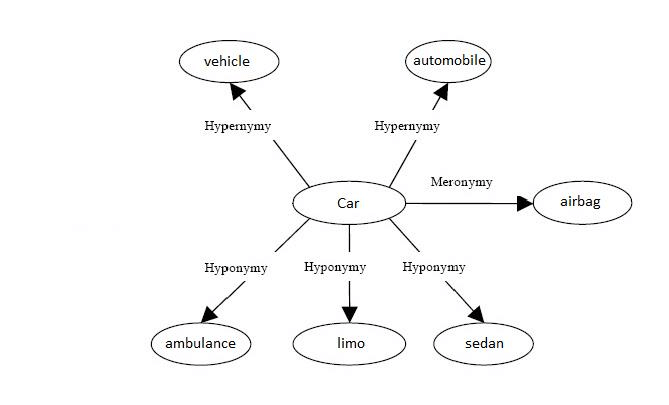
\includegraphics[height=200pt,width=330pt]{img/chapter2/wordnet.jpg}
            \caption{Synset du WordNet de l'Anglais}
            \label{synset}
        \end{figure}
    
    
    \subsection{Plongement de mots (Word embedding)}
    
     \textcolor{red}{Le plongement de mots (word embedding) est une technique qui permet de représenter les mots sous forme d'un vecteur de nombres réels grâce à un apprentissage fait sur un ensemble de mots, ce qui facilite l'anayse sémantique des mots.\\
    Les plongements de mots constituent une méthode pour faire face à un problème récurrent en intelligence artificielle, soit celui de la dimension. En effet, la représentation de mots avec les méthodes traditionnelles (bag of words) représentaient les mots avec un vecteur contenant tout le dictionnaire. En revanche la technique des word embeddings diminue le nombre de ces dimensions, facilitant ainsi les tâches d'apprentissage impliquant ces mots.}
    
    
    \subsubsection{Techniques d'apprentissage}
    
     \textcolor{red}{Il existe principalement deux techniques de word embeddings selon \cite{we1}} :
    
    \begin{itemize}
    \item  \textcolor{red}{La première appelée « Continuous Bag of Words » (CBOW), qui entraîne le réseau de neurones pour prédire un mot en fonction de son contexte, c’est à dire les mots avant/après dans une phrase.\\
    Dans le processus de CBOW, trois couches sont utilisées : la couche d'entrée correspond au contexte, la couche cachée correspond à la projection de chaque mot de la couche d'entrée dans la matrice de poids qui elle même  est projetée sur la troisième couche qui est la couche de sortie.\\ }
   
        \begin{figure}[H]
            \centering
            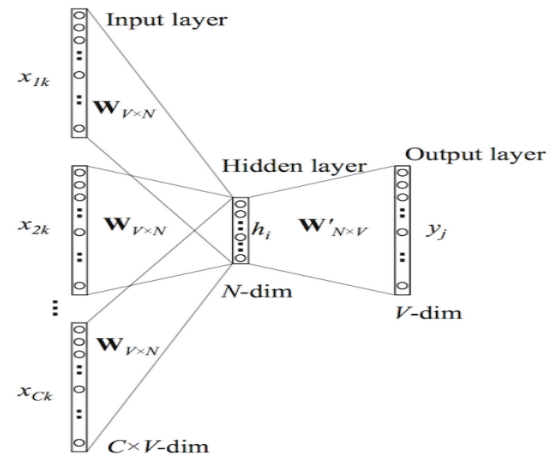
\includegraphics[height=250pt,width=300pt]{img/chapter2/Cbow.png}
            \caption{Réseau de neurones CBOW}
        \end{figure}
        
    
     \item  \textcolor{red}{Dans la seconde méthode, c'est le contraire des modèles CBOW: le modèle essaie de prédire le contexte en fonction du mot. C’est la technique du « skip-gram ». En effet, la couche d'entrée correspond au mot cible
     et la couche de sortie correspond au contexte. Ainsi, Skip-Gram cherche la prédiction du contexte étant donné un mot au lieu de la prédiction d'un mot étant donné son contexte comme c'est le cas pour CBOW.\\}
    
     \begin{figure}[H]
        \centering
        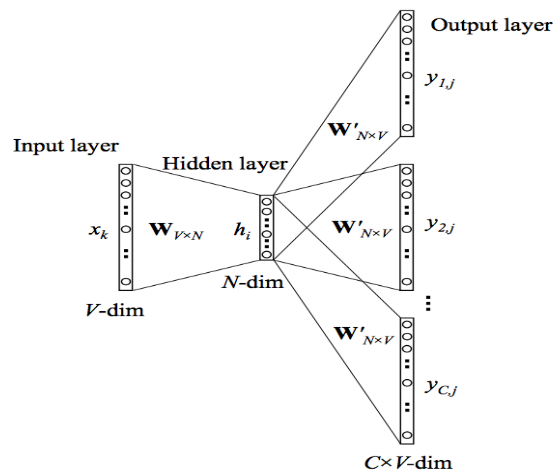
\includegraphics[height=250pt,width=300pt]{img/chapter2/Skip-Gram.png}
        \caption{Réseau de neurones Skip-Gram}
    \end{figure}
    
    \end{itemize}

    \subsubsection{Domaines d'application}
     \textcolor{red}{Grâce au gain en terme de dimensionalité, l'utilisation des plongements de mots (Word embedding) a permis de faciliter la tâche d'apprentissage dans la traduction automatique \cite{we2} en permettant une analyse des bigrammes et trigrammes, ce qui rend la traduction plus contextuelle.\\
    L'analyse des sentiment en a aussi profité, car elle n'a plus besoin de corpus annoté par un expert pour faire l'apprentissage \cite{we3} et la reconnaissance vocale qui a bénéficié d'une réduction des coûts et du temps de collecte et d'annotation de corpus \cite{we4}.}
       
 
    \subsection{Word2Vec}
     \textcolor{red}{Word2vec est un réseau de neurones à deux couches qui traite des documents texte. Son entrée est un corpus de textes et sa sortie est un ensemble de vecteurs: de caractéristiques pour les mots de ce corpus. Bien que Word2vec ne soit pas un réseau de neurones profond, il transforme le texte en une forme numérique que les réseaux profonds peuvent comprendre. Le but et l'utilité de Word2vec est de regrouper les vecteurs de mots similaires dans un espace vectoriel. Autrement dit, il détecte les similitudes mathématiquement. Word2vec crée des vecteurs qui sont des représentations numériques distribuées d'entités de mots, des caractéristiques telles que le contexte de mots individuels; tout cela est fait sans intervention d'un expert.\\}
    
    \subsubsection{Processus d'apprentissage}
    
     \textcolor{red}{Avec suffisamment de données, d'utilisation et de contextes, Word2vec peut faire des prédictions très précises sur la signification d'un mot en fonction des exemples passés. Ces prédictions peuvent être utilisées pour établir l'association d'un mot avec d'autres mots (par exemple, «homme» est un «garçon», «femme» est une «fille»), ou regrouper des documents et les classer par sujet. Ces clusters peuvent constituer la base de la recherche dans le domaine du traitement automatique du langage naturel.\\ 
    La sortie du réseau de neurones Word2vec est un vocabulaire dans lequel chaque élément est associé à un vecteur, qui peut être introduit dans un réseau d'apprentissage en profondeur ou simplement interrogé pour détecter les relations entre les mots. En mesurant la similitude de cosinus, aucune similitude est exprimée sous la forme d'un angle de 90 degrés, alors que la similarité totale de 1 est un angle de 0 degré, un chevauchement complet; c'est-à-dire que Algérie est égale à Algérie, tandis que algérien a une distance cosinus de 0.727976 par rapport à Algérie, qui est la plus petite distance par rapport aux autres mots. Voici une liste de mots associés à "Algeria" en utilisant Word2vec, par ordre de proximité }:
    
    \begin{table}[h!]
        \centering
                 \begin{tabular}{|l|c|r|}
                    \hline
                    Mot & Distance de cosinus\\
                    \hline
                    Algerian & 0.727976 \\
                    Morocco & 0.705196 \\
                    Tunisia & 0.698015 \\
                    Cameroon & 0.651363 \\
                    Gabon & 0.643677 \\ 
                    Algerians & 0.630602 \\
                    Senegal & 0.630219 \\
                    Ivory Coast & 0.627544 \\
                    Angola & 0.620858 \\
                    Burkina Faso & 0.617796 \\
                    \hline
                 \end{tabular}
             \caption{Exemple du vecteur de similarité du mot "Algeria".}
             \label{table:1}
         \end{table}
             
    
    
    
    \subsubsection{Domaines d'application de Word2vec}
     \textcolor{red}{Les applications de Word2vec s'étendent au-delà de l'analyse des phrases. Il peut être appliqué aussi bien aux gènes, au code, aux goûts, aux playlists, aux graphiques de médias sociaux et à d'autres séries verbales ou symboliques dans lesquelles des modèles peuvent être discernés, puisque les mots sont simplement des états discrets comme les autres et nous cherchons simplement les probabilités de transition entre ces états.}
    
    

\section{Résumé automatique}
    \subsection{Définition}
    Le résumé automatique consiste à diminuer le contenu d'un document/texte avec un programme informatique. Le texte résultant (résumé) devrait contenir les idées les plus importantes du texte original.

    \emph{"La synthèse de texte est un processus qui consiste à distiller les informations les plus importantes d'une source pour produire une version abrégée"}\footnote{Traduction par les auteurs de ce mémoire}\cite{aats}(Page 1)\\

    Cette technique est de plus en plus nécessaires pour répondre à la croissance exponentielle des quantités  de données textuelles disponibles sur internet pour mieux reconnaître les informations pertinentes et pour les consommer plus rapidement.

    Dans un livre de 2014 intitulé «Automatic Text Summarization»\cite{atsjmtm}(Pages 4-5), l'auteur à cité 6 raisons pour lesquelles nous avons besoin d'outils pour le résumé automatique:

    \begin{itemize}
        \item Les résumés réduisent le temps de lecture.
        \item Lors de la recherche de documents, les résumés facilitent le processus de sélection.
        \item L'utilisation de cette technique permet d'augmenter le nombre de textes traités.
        \item Le résumé automatique améliore l'efficacité de l'indexation.
        \item Les algorithmes de résumé automatique sont moins biaisés que les synthétiseurs humains.
        \item Les résumés personnalisés sont utiles dans les systèmes de Question/Réponse car ils fournissent des informations personnalisées.
    \end{itemize}

    \subsection{Domaines d'application}    
    Il existe de nombreuses raisons et utilisations des résumés automatiques. Un exemple qui pourrait facilement venir à l'esprit est de créer un résumé d'un article de presse, mais il y a beaucoup plus de cas de résumés de texte que nous pouvons rencontrer tous les jours.

    Voici quelques exemples quotidiens de résumés de textes:
    \begin{itemize}
        \item Grandes lignes (prise de notes)
        \item Synopsis (scénario d'un film)
        \item Avis (Livre, article..)
        \item Biographie (Curriculum Vitae, nécrologie)
        \item Bulletins (prévisions météo)
        \item Histoire (chronologies des événements)
    \end{itemize}

    \subsection{Résumé extractif}
        Cette approche de résumé automatique implique la sélection de phrases à partir d'un document source pour constituer un nouveau texte (résumé). Les techniques consistent à classer la pertinence des phrases afin de retenir celles qui sont les plus importantes pour garder le sens et la signification du texte original.

        La pertinence d'une phrase est calculée à base de plusieurs caractéristiques (Features). Certaines de celles-ci sont\cite{ratsa} :
        
        \begin{itemize}
            \item \textbf{Titre:} Les mots de titre apparaissant dans une phrase pourraient suggérer que la phrase contient des informations importantes
            \item \textbf{Position de la phrase:} Les phrases de début dans un document habituellement décrivent les principales informations concernant document.
            \item \textbf{Longueur de la phrase:} Les phrases trop courtes peuvent contenir moins d'informations et les longues phrases ne sont pas appropriées à représenter le résumé.
            \item \textbf{Poids d'un mot/terme:} Mots ou termes qui ont une occurrence élevée dans un document sont utilisés pour déterminer l'importance d'une phrase.
            \item \textbf{Noms propres/Entités nommées:} les noms de personnes, organisations, lieux, etc. sont considérés comme porteurs d'informations importantes.
        \end{itemize}   

        \subsubsection{État de l'art du Résumé extractif}
        \textbf{•La méthode basée TF-IDF\footnote{Term Frequency-Inverse Document Frequency, méthode de pondération souvent utilisée en recherche d'information.}:}
            Les phrases sont classées en fonction de la fréquence du terme et de l'inverse de la fréquence du document \cite{tfidf}. La similarité entre le vecteur de requête et les vecteurs de phrases est calculée puis les phrases les plus importantes sont incluses dans le résumé. L'inconvénient est  la Redondance dans le résumés.\cite{surveysummarization}
            
        \textbf{•La méthode basée sur apprentissage automatique supervisé:} Les phrases sont classées sur la base de l'inclusion de phrases récapitulatives et de l'exclusion de phrases résumées. La classification est basée sur les caractéristiques de la pertinence des phrases dans le résumé. Les probabilités de classification sont faites sur la base de la technique statistique en utilisant la règle de Bayes. Dans ce cas, la redondance sera peut être réduite mais cette méthode reste complexe.\cite{surveysummarization}
            
        \textbf{•La méthode basée sur le Clustering\footnote{Le partitionnement de données, méthode d'analyse de données, vise à diviser un ensemble de données en différents « paquets » homogènes, chaque sous-ensemble partageant des caractéristiques communes.}:} Ces documents sont représentés en utilisant le TF-IDF de dizaines de mots. La fréquence de terme utilisée dans ce contexte est le nombre moyen d'occurrences (par document) dans le cluster. La valeur IDF est calculée sur la base du corpus entier. Le synthétiseur prend des documents déjà groupés en entrée. Chaque cluster est considéré comme un thème.
        Le thème quant à lui est représenté par des mots avec leurs fréquences d’occurrences.\\
        La sélection de la phrase est basée sur la similarité des phrases au thème du cluster. Le facteur suivant qui est pris en compte pour la sélection de la phrase est l'emplacement de la phrase dans le document (Li). Le dernier facteur qui augmente la score d'une phrase est sa similitude avec la première phrase du document auquel elle appartient (Fi).\\
        L'avantage du clustering est qu'il peut être utilisé pour grouper des phrases similaires dans plusieurs document\cite{surveysummarization}.
            
        \textbf{•La méthode basée Logique Floue\footnote{Formalisée par Lotfi Zadeh en 1965, elle consiste à tenir compte de divers facteurs numériques pour aboutir à une décision qu'on souhaite acceptable.}:} Le système flou considère les caractéristiques des phrases telles que la longueur de la phrase, le mot du titre, les mots-clés, .etc\cite{10}. Il assigne un score aux phrases et extrait les plus importantes sur la base des valeurs assignées.\\
        L'avantage de cette méthode consiste en la facilité de l'extraction des caractéristiques qui servent à calculé le score qui sert, à son tours, comme entrée à \emph{Fuzzifier}, mais la performance de cette approche reste limitée\cite{surveysummarization}.

    \subsection{Résumé abstractif}
        L'approche de résumé automatique abstractive quant à elle, consiste en la génération de phrases entièrement nouvelles. Cette méthode est plus difficile, mais c'est aussi l'approche utilisée par l'humain. Elle est basée sur la sélection et la compression du contenu original.

        Récemment, les méthodes d'apprentissage en profondeur ont montré des résultats prometteurs pour le résumé automatique. Des approches ont été proposées inspirées par l'application de méthodes d'apprentissage en profondeur pour la traduction automatique.

        Principalement basées sur les Réseaux de neurones récurrents, ces dernières ont pu montrer des performances et des résultats assez impressionnants, comme on peut le constater dans \cite{atsuss} et \cite{ruch} où plusieurs nouveaux modèles basés sur l'apprentissage profond ont été proposés qui surpassent statistiquement toutes les autres approches abstractives.

        \subsubsection{État de l'art du Résumé abstractif}
        \textbf{•Méthode basée sur les arbres:} Elle utilise un arbre de dépendance pour représenter le texte d'un document. Sur la base des relations entre les sous-arbres les phrases similaires sont sélectionnées et le résumeur génère le résumé final \cite{5}.
            
        \textbf{•Méthode basée sur un modèle:} Elle utilise un modèle pour représenter le document. Les modèles linguistiques et les règles d'extraction sont utilisées pour identifier les extraits du texte les plus pertinents\cite{5}.

        \textbf{•Méthode basée sur l'ontologie:} Dans cette méthode, \textcolor{red}{il est question d'utiliser des ontologies dans le processus de résumé automatique \cite{ram}.!!}
 
        

\section{Catégorisation de textes}
    \subsection{Définition}
    La catégorisation de textes a pour objectif de regrouper les textes similaires, c'est à dire thématiquement proches. L'intérêt d'une telle démarche est d'organiser les connaissances de façon à pouvoir effectuer, par la suite, une recherche ou une extraction d'information efficace. Elle est largement étudiée dans différentes communautés tels que le Data Mining, les bases de données, l'apprentissage automatique et la recherche d'informations.

    \subsection{Domaines d'application}
    Plusieurs applications dans lesquelles la catégorisation de textes est couramment utilisée, on peut citer:

    \textbf{•Filtrage et organisation des informations d'actualités:} avec les quantités énormes de d'informations d'actualités en ligne, il est très difficile de catégoriser ces dernières manuellement, mais cela est possible grâce aux algorithmes de classifications. 

    \textbf{•Organisation des documents:} aider à la catégorisation de documents, un exemple d'application est l'ensemble des fichiers d'un ordinateur où il s'agit de distinguer les fichiers \emph{log}, \emph{système}, etc.

    \textbf{•Exploration des opinions:} souvent utilisée pour la catégorisation des commentaires sur les réseaux sociaux.

    \textbf{•Catégorisation des emails et filtrage des spams:} reconnaître l'objet de l'email ou déterminer les courriers indésirables de manière automatisée.
     
    \subsection{Technique de classifications de textes}
    De nombreuse techniques ont été conçues pour la catégorisation des textes. Puisqu'il est possible de modéliser ces derniers comme des données quantitatives généralement avec des fréquences de termes, la plupart des méthodes appliquées aux problèmes quantitatifs sont également applicables.\\    
    Quelques une de ces techniques on été citées dans \cite{stca}:

    \begin{itemize}
        \item Arbres de décisions: la division hiérarchique de l'espace de données dans les arbres de décisions permet de créer des partitions de classes qui sont plus asymétriques en termes de distribution de leurs classes.

        \item Base de règles: déterminer les modèles de mots le plus susceptibles d'être liés aux différentes classes, basé sur un ensemble de règles dans lesquelles le coté gauche correspond à un motif de mot, et le coté droit à une étiquette de classe.

        \item SVM: tentent de partitionner l'espace de données en utilisant des fonctions linéaires et non linéaires pour séparer les classes.

        \item Réseau de neurones: avec l'utilisation des caractéristiques des mots, tout comme les SVMs les RNs essaient de trouver la limite la plus optimale entre les classes.

        \item Autres: presque tous les algorithmes de classification peuvent être adaptés aux données textuelles, tel que les algorithmes génétiques, etc.
    \end{itemize}


    \subsection{Catégorisation d'articles de presse}
     L’étude de la presse en ligne est devenue ces derniers temps un enjeu de recherche, et le nombre phénoménal de journaux, magazines et blogs sur internet qui ne cessent d'augmenter a fait de la catégorisation d'articles de presse l'une des tâches les plus importantes de la catégorisation de textes. Il s'agit de ranger des articles dans des classes, idéalement convenables, suivant une problématique donnée, souvent le domaine traité par l'article, comme Politique, Sport, Religion, Économie, etc.

    \subsubsection{État de l'art de la catégorisation d'articles de presse}
    
      \textcolor{red}{De nombreux travaux de recherches ont été faits dans la catégorisation de textes mais ce qui est plus intéressant pour nous c'est de prospecter ceux destinés à la catégorisation des articles de presse \cite{itemetat0}, parmi ceux-là on retrouve} :
     
     \begin{itemize}
        
     \item  \textcolor{red}{Thorsten Joachims introduit les machines à vecteurs de support (Support vector machine) pour la catégorisation de textes. Il fournit à la fois théorique et preuve empirique que les SVM sont très bien adaptés pour la catégorisation de textes \cite{itemetat1}}. 
     
     \item  \textcolor{red}{Susain Dumais compare l'efficacité de cinq algorithmes d'apprentissage automatique différents pour la catégorisation en termes de vitesse d'apprentissage, classement en temps réel, la vitesse et la précision de la classification. Il examine également la taille de l'ensemble d'entraînement et la représentation de documents alternatifs \cite{itemetat2}}.
     
     \item  \textcolor{red}{Chee Hong a expérimenté une approche automatisée pour classer les articles de presse en ligne en utilisant la méthode de classification SVM. L'utilisation de SVM a donné de bons résultats quand les données d'apprentissage (Articles de presse) étaient suffisants \cite{itemetat3}}.
      
     \item  \textcolor{red}{Krishanalal a développé le classifieur d'articles de presse intelligent et l'à expérimenté en ligne pour les catégories Sports, Finances et politique. L'approche novatrice combinant deux puissants algorithmes, modèle de Markov caché et SVM, dans le domaine de classement en ligne des articles de presse a fourni de bons résultats par rapport aux méthodologies existantes. Par l'introduction de plusieurs techniques de prétraitement, ils ont pu améliorer la précision du classifieur \cite{itemetat6}}.
     
     \item  \textcolor{red}{Mita K. Dalal a travaillé sur la classification de textes et l'extraction des caractéristiques; il a conclu que les étapes de pré-traitement et de sélection des fonctions ainsi que le choix des données d'apprentissage jouent un rôle crucial dans pour l'amélioration de la précision \cite{itemetat7}}. 
     
     \item  \textcolor{red}{Adgar a proposé une approche pour classer les articles de presse et l'a décomposée en 3 étapes: prétraitement du texte, extraction de caractéristiques basée sur TF-IDF et la classifiation basée sur SVM.
     Il a choisi SVM, car ceux-ci peuvent supporter données avec des dimensions élevées \cite{itemetat8}}.
     
     \end{itemize}
        

\section{La traduction automatique}
La traduction est une activité en croissance très rapide de nos jours \cite{tradstat}. C'est un moyen actif de transférer la culture et la langue en communicant avec autrui \cite{tradcom}. Son aspect principal est de faire passer un message ou un texte rédigé d'une langue vers une autre en respectant le contexte et la grammaire.\\
Depuis très longtemps, la traduction automatique s'inscrit dans une recherche appartenant au domaine du traitement automatique du langage naturel.
    \subsection{Définition}
    La traduction automatique est la procédure par laquelle un ordinateur évalue un contenu source en entrée dans une langue donnée et délivre un contenu cible dans une langue différente en respectant les aspects lexicaux, syntaxiques, sémantiques et morphologiques des deux langues.
    \subsection{Types de traduction automatique}
    Les traducteurs automatiques se distinguent dans les catégories suivantes en :
        \subsubsection{Traducteur automatique basé dictionnaire}
        Dans ce type de traducteur, historiquement l'approche la plus ancienne et obsolète, la traduction automatique était basée sur les traductions des dictionnaires multilingues ordinaires, c'est a dire la traduction des mots du texte en entrée mot par mot en ne prenant pas en considération le sens des phrases. Il est a noter que les recherches dans le dictionnaire peuvent être faites avec ou sans l'utilisation des outils de langages dans l'analyse.
        \subsubsection{Traducteur automatique à base de règles de production}
        Dans ce type de traduction automatique, le traducteur prend en compte les données étymologiques des langues des documents en entrée et le document cible fondamentalement récupéré de 
        lexiques et structures de phrases couvrant les règles sémantiques, morphologiques et syntaxiques principales de chaque langue individuellement. L'acquisition des phrases composant la langue du document source par le traducteur permet de produire des phrases cibles dans la langue du document cible sur le principe d'analyses morphologique, syntaxique et sémantique des deux langues.
        Les principaux travaux utilisant les bases de règles pour la traduction ont été créés au milieu des années 1970\cite{surveyTraduction}.
        Les traducteurs automatiques à base de règles de production sont capables de produire des traductions avec une qualité raisonnable, mais la construction du système prend beaucoup de temps et de main-d'œuvre parce que ces ressources linguistiques doivent être fabriquées à la main.De plus, il est très difficile de corriger l'entrée ou d'ajouter de nouvelles règles au système pour générer une traduction\cite{jean}.
        \subsubsection{Traducteur automatique à base d'exemples}
        L'approche à base d'exemples repose sur un ensemble de phrases traduites préalablement. Lors de la traduction, le processus vérifie si la phrase à l'entrée est parmi les exemples; dans le cas positif, il fournit directement sa traduction, sinon il s'inspire d'autres phrases contenant un ou plusieurs ensembles de mots similaires et fournit la traduction de ces mots selon les exemples dont il dispose\cite{setif}.
        \subsubsection{Traducteur automatique basé connaissances}
        Ce type de traducteur automatique se concentre sur l'aspect lexical que représente un domaine défini (propre à un seul domaine), comme par exemple, un traducteur pour les articles de recherches, médecine, etc\cite{surveyTraduction}.
        \subsubsection{Traducteur automatique basé sur un corpus}
        La traduction automatique basée sur le corpus (CBMT) est générée sur l'analyse des corpus de textes bilingues. Cette technique utilisée depuis 1989 se base sur un corpus de traduction pour la machine. Cette technique a dominé sur les autres compte tenu de son exactitude, notamment à l'ajout d'exemples au système qui peut améliorer ses performances puisqu'il est basé sur les données, bien que l'accumulation et la gestion de l'énorme corpus de données bilingues puisse également être coûteuses\cite{jean}.
        \subsubsection{Traducteur automatique basé contexte}
        La traduction automatique basée contexte est un nouveau paradigme pour la traduction automatique basée corpus qui nécessite un vaste corpus de textes cibles monolingues et un dictionnaire bilingue complet. CONTRAST \cite{8} et REFTEX \cite{9} sont deux exemples de systèmes de traduction automatique basée contexte.


\section{Conclusion}
Dans ce chapitre, nous avons essayé de faire le tour des techniques du Traitement Automatique du Langage Naturel. Nous avons d'abord présenté cette science, son importance et ses domaines d'application. Ensuite, nous avons examiné l'état de l'art de chaque technique en expliquant les processus et les méthodes. Enfin, nous avons passée rapidement en revue certaines applications actuelles du TALN.
Le prochain point à aborder quant à lui, présentera notre contribution, la conception générale de la solution proposée et ses différentes fonctionnalités.  